\section{问答附录}

\begin{frame}{附录 A · 四类查询的正确性}
\fontsize{11}{14}\selectfont
\textbf{充分性：}核心距离不超过 $k-a-b$，接回起点与终点的 $a,b\in\{0,1\}$ 跳边，就得到长度不超过 $k$ 的行走；去环后仍有合法路径。\par\vspace{2mm}
\textbf{必要性：}合法路径的覆盖外起点首步必进入 $S$，覆盖外终点末步必来自 $S$。因此路径必经四类查询枚举的一对核心点，其最短核心距离满足剩余预算。\par\vspace{2mm}
\textbf{边界处理：}先处理 $s=t$；核心对角线保留零距离。两个外部端点共享一个核心邻居时也能正确接受。$k=1$ 可直接查边，本项目索引实验使用 $k\ge2$。
\Key{任意合法路径均对应一个满足预算的核心点对。}
\end{frame}

\begin{frame}{附录 B · 固定 $k$ 的索引与多 $k$ 查询}
假设在 $k=6$ 时建索引：\par\vspace{2mm}
$d(u,v)=2$ 与 $d(u,v)=4$ 都编码成 \T{01}，即“$d\le4$”。\par\vspace{2mm}
改问 $k=3$ 时，两者答案不同，原码却无法区分。\par\vspace{3mm}
原文 §4.4 讨论多 $k$ 的扩展；保存完整核心距离与三档码是不同设计。本项目 $k=2,4,6$ 分别编码，也分别构造预算相关边界。
\Key{固定 $k$ 下仍须区分两个预算：\T{Case 2/3 用 $k-1$，Case 4 用 $k-2$}。}
\end{frame}

\begin{frame}{附录 C · 原文 $(h,k)$-Reach 的空间—时间取舍}
\fontsize{11}{14}\selectfont
\textbf{$h$-hop 顶点覆盖：}每条长度为 $h$ 的路径至少含一个覆盖点。核心可以更小，但外部端点可能要走 $1\ldots h$ 跳接入核心。\par\vspace{2mm}
核心预算相应变为 $k-i-j$，需要保留更多距离阈值；原文定义给出 $h<k/2$。\par\vspace{2mm}
Nasa 的 $h=2,\mu=7$ 满足条件：覆盖 $1841\to1223$，百万查询从 $18.23\to39.48$ms。$\mu$ 为图上最短路径长度中位数。
\Key{更小的覆盖减少索引规模，同时增加端点接入核心的搜索开销。}
\end{frame}

\begin{frame}{附录 D · 核心编码是对照因素，单独控制}
\fontsize{11}{14}\selectfont
原文 §4.3 已讨论压缩。我们实现两位类别打包 CSR 与按行稀疏/稠密的 Hybrid，用作物理表示对照；\textbf{主图比较相同 Hybrid 上剪枝前后}。\par\vspace{2mm}
稀疏行载荷约 $4r+\lceil r/4\rceil$ 字节，稠密行 $\lceil |S|/4\rceil$ 字节。计入元数据后，混合布局不如两种全局格式时整体回退。\par\vspace{2mm}
原边界在所有新对照中均预先转为核心 ID，使用相同答案核。CSR 求交另有原边界和剪枝边界两个版本。
\Key{分别比较相同编码和相同查询方式下的剪枝效果。}
\end{frame}

\begin{frame}{附录 E · 部署空间、证书暂存与预处理分摊}
{\fontsize{9}{11}\selectfont\centering\begin{tabular*}{\textwidth}{@{\extracolsep{\fill}}lrrrrr@{}}\toprule
图 & 原边界/MiB & 剪枝/MiB & 总部署/MiB & 构建/s & 证书/MiB\\\midrule
Wiki-Vote & 0.10 & 0.17 & 2.01 & 0.10 & 2.52\\
Gnutella31 & 0.71 & 1.42 & 22.99 & 2.23 & 155.47\\
Email-EuAll & 3.37 & 6.63 & 34.74 & 5.04 & 314.92\\
\bottomrule\end{tabular*}\par}\par\vspace{2mm}
\fontsize{10.5}{13}\selectfont
总部署包含核心索引、节点映射和边界。证书用于离线构建，完成后可释放。Email 的核心距离暂存矩阵约为 1.23 GiB。\par\vspace{2mm}
原边界两个预算复用数组；剪枝后的预算列表分别保存，因此可能增加空间。
\Key{面向静态图上的重复查询，\T{预处理与额外存储是明确代价}。}
\Micro{Wiki $k=4$：按构建时间 0.10s 与当前平均查询节省估算，约 1.92 百万次查询可分摊构建开销。}
\end{frame}

\begin{frame}{附录 F · 不同 $k$ 下，结构相关收益也会变化}
\centering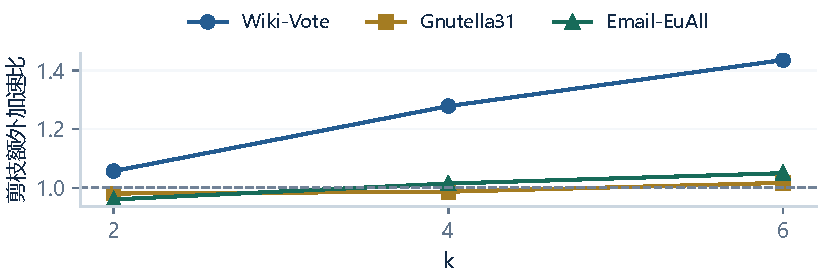
\includegraphics[width=.98\textwidth,height=44mm,keepaspectratio]{k_pruning.pdf}\par
\Key{每个 $k$ 分别建立两层预算边界；收益受阈值包含关系与原始查询工作共同影响。}
\end{frame}

\begin{frame}{附录 G · 更换覆盖构造，结论是否只依赖一次选择？}
\centering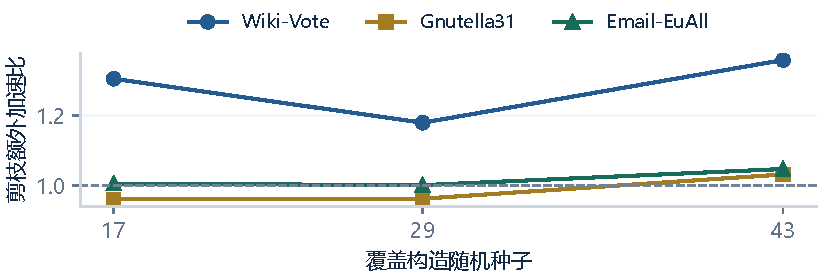
\includegraphics[width=.98\textwidth,height=44mm,keepaspectratio]{cover_pruning.pdf}\par
\Key{覆盖种子 17 / 29 / 43 全部保留，未按测试计时挑选覆盖；Wiki 在三次覆盖下均有收益。}
\end{frame}

\begin{frame}{附录 H · 单侧与双侧剪枝的时间消融}
\centering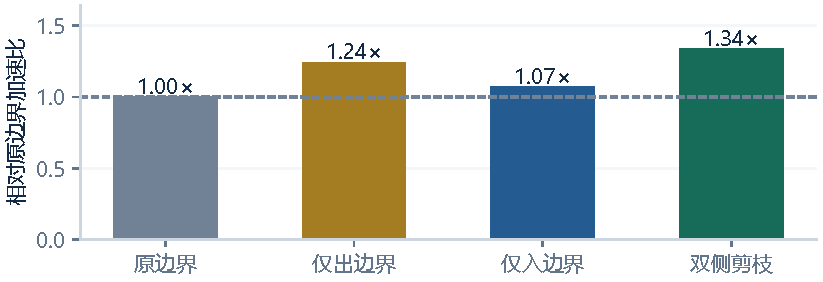
\includegraphics[width=.98\textwidth,height=44mm,keepaspectratio]{ablation.pdf}\par
\Key{出、入边界贡献不同；双侧同时保留阈值见证，再由实际计时判断整体收益。}
\end{frame}

\begin{frame}{附录 I · 所有图与 $k$ 的完整查询结果}
{\fontsize{8.5}{11}\selectfont\centering\begin{tabular*}{\textwidth}{@{\extracolsep{\fill}}llrrrrrr@{}}\toprule
图 & $k$ & Join & +剪枝 & 加速 & Hybrid & +剪枝 & 加速\\\midrule
Wiki-Vote & 2 & 0.550 & 0.557 & 0.99 & 0.425 & 0.403 & 1.06\\
Wiki-Vote & 4 & 0.429 & 0.379 & 1.13 & 0.246 & 0.191 & 1.28\\
Wiki-Vote & 6 & 0.363 & 0.302 & 1.20 & 0.212 & 0.145 & 1.43\\
Gnutella31 & 2 & 0.263 & 0.262 & 1.00 & 0.281 & 0.287 & 0.98\\
Gnutella31 & 4 & 0.344 & 0.349 & 0.98 & 0.357 & 0.361 & 0.99\\
Gnutella31 & 6 & 0.516 & 0.516 & 1.00 & 0.272 & 0.267 & 1.02\\
Email-EuAll & 2 & 0.416 & 0.423 & 0.98 & 0.420 & 0.437 & 0.96\\
Email-EuAll & 4 & 0.366 & 0.379 & 0.97 & 0.251 & 0.247 & 1.01\\
Email-EuAll & 6 & 0.339 & 0.333 & 1.02 & 0.232 & 0.221 & 1.05\\
\bottomrule\end{tabular*}\par}
\Micro{时间单位：$\mu$s/查询。Join / Hybrid 各自配对比较，避免把换编码的收益算到剪枝上。}
\end{frame}

\begin{frame}{附录 J · 后续研究与本项目分别优化什么？}
\fontsize{11}{14}\selectfont
\textbf{VCRea / VCRea$^+$（Tang 等，2023）}\par
以顶点覆盖构造两跳距离标签，给高出度点扩展 out-label、高入度点扩展 in-label，将标签对比较次数限制在至多 $d^2$。增加标签是一种空间与枚举代价取舍。\par\vspace{3mm}
\textbf{阈值支配剪枝（本项目）}\par
不增加距离精度，按现有两档阈值集合的包含关系消去冗余邻居；代价是边界构建及额外列表。\par\vspace{2mm}
近期 CSUR 综述单列 hop-constrained 语义，说明普通可达索引不能直接替代跳数约束。
\Key{VCRea 扩展距离标签；本项目研究固定 K-Reach 索引上的边界约简。}
\end{frame}

\begin{frame}{附录 K · 双侧约简的正确性}
\fontsize{11}{14}\selectfont
原出/入边界为 $A,B$，保留代表为 $A',B'$。任意合法核心对 $(y,v)$，满足 $d(y,v)\le b$。\par\vspace{2mm}
\textbf{替代源侧：}有 $x\in A'$，使 $R_b(y)\subseteq R_b(x)$。因此 $v\in R_b(x)$，即 $d(x,v)\le b$。\par\vspace{2mm}
\textbf{替代终侧：}有 $v'\in B'$，使 $L_b(v)\subseteq L_b(v')$。既然 $x\in L_b(v)$，就有 $d(x,v')\le b$。\par\vspace{2mm}
保留边界又是原边界的子集，所以不存在新增的错误成功见证。单侧分支只做相应的一次替代。
\Key{两侧必须用\T{相同剩余预算}，且终侧用前驱集合；普通可达或任意 SCC 代表不满足此条件。}
\end{frame}

\begin{frame}{附录 L · 构建方法与查找次数的变化}
\fontsize{10.5}{13}\selectfont
按集合大小降序处理邻居；已被保留集合包含就消去。反射性给出必要条件：\par
\[
R_b(y)\subseteq R_b(x)\ \Rightarrow\ d(x,y)\le b .
\]
先做该常数检查，再验证位集合包含。真实图审计使用\textbf{直接整数距离}逐项核对被消去者与其保留代表，独立于位打包构建。\par\vspace{2mm}
潜在候选上界不会增加，但找到成功见证的顺序可能变化。主实验及覆盖补充中，有 5 条查询的实际查找次数增加。
\Key{代表点可能出现在更后的位置，因此部分查询会在更多次检查后找到成功见证。}
\end{frame}

\begin{frame}{附录 M · 受控合成图上的机制验证}
\centering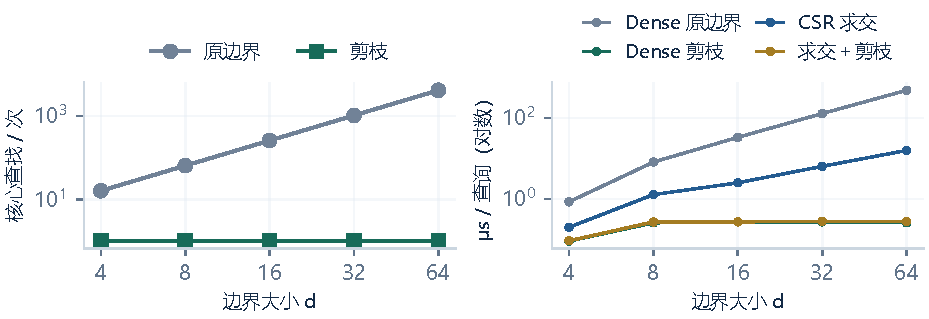
\includegraphics[width=.98\textwidth,height=50mm,keepaspectratio]{synthetic.pdf}\par
\Key{嵌套边界负例：原查找 $d^2$ 次，约简后 1 次。\T{固定全稠密 lookup 也有候选增长问题。}}
\end{frame}

\begin{frame}{参考文献}
\fontsize{9.5}{12}\selectfont
\begin{enumerate}\setlength\itemsep{3mm}
\item J. Cheng, Z. Shang, H. Cheng, H. Wang, J. X. Yu. \textbf{K-Reach: Who is in Your Small World.} \emph{PVLDB} 5(11):1292–1303, 2012. \href{https://doi.org/10.14778/2350229.2350247}{doi:10.14778/2350229.2350247}.
\item X. Tang, J. Zhou, Y. Shi, X. Liu, K. Lin. \textbf{Efficient Processing of k-Hop Reachability Queries on Directed Graphs.} \emph{Applied Sciences} 13(6):3470, 2023. \href{https://doi.org/10.3390/app13063470}{doi:10.3390/app13063470}.
\item C. Zhang, A. Bonifati, M. T. \"Ozsu. \textbf{Indexing Techniques for Graph Reachability Queries.} \emph{ACM CSUR} 58(6), Article 156, 2026; online Dec. 2025. \href{https://doi.org/10.1145/3776737}{doi:10.1145/3776737}.
\item J. Leskovec, A. Krevl. \textbf{SNAP Datasets}. \href{https://snap.stanford.edu/data/}{snap.stanford.edu/data/}.
\end{enumerate}
\end{frame}

